\documentclass[article]{report} % Type of document

\usepackage[utf8]{inputenc}    		 	% Encoding
\usepackage[english]{babel}			% Language
\usepackage{geometry}           			% Page margin
\usepackage{graphicx}           			% For images
\usepackage{newcent}            			% Font
\usepackage{color}              			% Colors
\usepackage{listings}           			% Lists
\usepackage[footnote, nolist]{acronym}	% Acronyms
\usepackage[absolute, overlay]{textpos}	% Text positioning

\usepackage{fancyhdr}          			 % We might have a need for them
\usepackage{float}
\usepackage{tabularx}

\usepackage{latexsym}
\usepackage{pdfpages}
\usepackage{tikz}
\usepackage{ifthen}
\usepackage{wrapfig}
\usepackage{textcomp}
\usepackage{multicol}

\setlength{\columnsep}{1cm}
\setlength{\TPHorizModule}{\paperwidth}	% Used for textblock
\setlength{\TPVertModule}{\paperheight}	% Used for textblock

\title {Book of specifications}
\parskip = 0.25cm              % Summary options (spaces between lines)

% Margin
\geometry{tmargin=2.5cm, bmargin=2cm, lmargin=2.5cm, rmargin=2cm}

\definecolor{blue}{rgb}{0.13,0.29,0.46}
\definecolor{red}{rgb}{1,0,0}
\definecolor{couleur_titre}{rgb}{0.20, 0.45, 0.80}
\definecolor{couleur_nom}{rgb}{0.11, 0.6, 0.18}

\renewcommand{\labelitemi}{$\bullet$}

% Title at the top of the page
\pagestyle{fancyplain} \chead{}\lhead{\textit{Team Dedalus}} \rhead{\textcolor{couleur_titre}{\emph{\textit{Project: Islands}}}}

\title {Specifications}
\author {Romain\and Renaud\and Aenora\and Erwan}
\date {}

%
% Document
%
\begin{document}
		\thispagestyle{empty}
  			\begin{titlepage} 
						\vspace*{5cm} 
  					\begin{center} 
  							{\huge{\textsc{Cahier des charges} \\ ~ \\{\large From}\\ ~\\ Team Dedalus \\ ~ \\ Islands}}
	  						\vspace*{10cm}
						\end{center}
  					\hfill {\large Romain \textsc{Biessy}}
  					\hfill {\large Renaud \textsc{Gaubert}}
  					\hfill {\large Aenora \textsc{Tye}}
  					\hfill {\large Erwan  \textsc{Vasseure}}
  			\end{titlepage} 
  	\renewcommand{\contentsname}{Table of contents}

  	\tableofcontents
  			\pagenumbering{arabic}
  			\newpage
				\chapter{\textcolor{blue}{Introduction}}%<- modifier la pagination
								Even though we didn't start coding, we still had six to seven group meeting to discuss about the project. And spent at least 15 hours speeking together.\newline
								However, the project's general gameplay was fixed unanimously on the first reunion. It will be a 3D RTS at the first person. Thus a mix between RTS and FPS. Creating a game has never been an easy task but, the game how we see could be described as ambitious. Nevertheless, our teamwork should not be underestimate.\\
								
								When we assigned the differents task to our members, we had in mind the idea that everybody should know how most of the game works and not only one member. Therfore, we had to split the project in a way that would help us later : modules. Thus even if we didn't begin to code the game, we have some kind of base. 								
								
  			\chapter{Gameplay}
						\section{Section 1}
							  \subsection{Sub 1}
				\chapter{Goals and interest}
						\section{Learning new Languages}
								Since half of the group are inexperienced programmers, one of the major goal of the project will be to learn about computer programming.\\
								
								Of course it won't be limited to C\#, because of the fact that we are working with OO, to ensure that everybody can understand the code, we will be using UML.\newline
								Also we will be discovering and thus learning about the following languages : 
								\begin{itemize}
										\item HTML5/CSS3 and PHP/MySQL with maybe some JavaScript for the website;
										\item XML because this is how the GUI layout will be written.
								\end{itemize}
															
								We will be using some OO well known principles such as inheritance and abstract class. We also might use Symfony2 (with Doctrine) for the website.
							  
						\section{Learning about web}
							  		Symfony is a PHP Web Development Framework. Thus it provides generic functionality and "helps" you writting good code. What i mean with good code is the fact that because of its own architecture organize your code.\\
							  		
							  		The power of symfony lies in the MVC organization. Indeed Symfony2 is developped in an architecture that separates the representation of information from the user's interaction with it.\newline
							  		 Thus when the user will try to access to a website URL, this URL will be submited to the router, which will then call the right PHP function which will then send variables, after processing the data relative to it's function, to a TWIG page which will then be displayed.
							  		 
						\section{Learning about 3d}
								As you might've already understood, we are using Mogre which is a scene-oriented, real-time, flexible 3D rendering engine 3d library.\newline
								The class library abstracts the details of using the underlying system libraries like Direct3D and OpenGL and provides an interface based on world objects and other high level classes.\\
								
								Thus, the user can choose between Direct3D and OpenGL without us having to rewrite the entire code for each libraries. As its name states, OGRE is "just" a rendering engine. As such, its main purpose is to provide a general solution for graphics rendering. Though it also comes with other facilities (vector and matrix classes, memory handling, etc.), they are considered supplemental. It is not an all-in-one solution in terms of game development or simulation as it doesn't provide audio or physics support, for instance.\\
								
								You should also know that having an experience with 3d is generally far more interesting than having an experience with 2d. Thus we decided to do some 3d.
								
								
					
						\section{Goals}
				\chapter{Behind the scene}
     				\section{Language \& Game design pattern}
     						Our project will be coded in \textbf{C\#} .NET 4.0 mainly because of the \ac{OOP} paradigm and also for the large choice there is about 3D engine and libraries. The OO let us use the \textbf{game state} pattern in order to structure the code. Basically, we consider our game as a stack of different states. Here is an example of a game state:
							\begin{figure}[h]
							\centering
							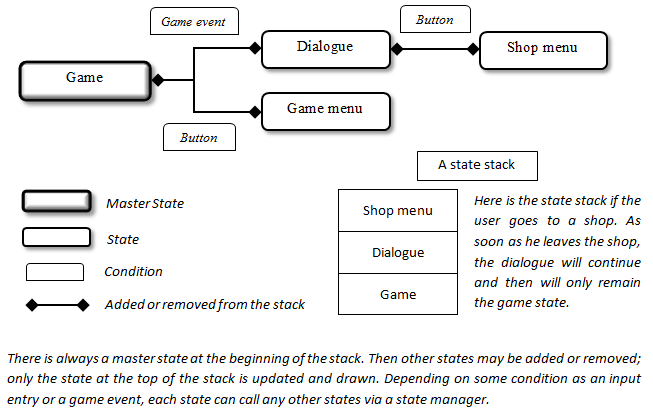
\includegraphics[height=242px]{Images/GameStateDesign.png}
							\it \\ There is always a master state at the beginning of the stack. Then other states may be added or removed; only the state at the top of the stack is updated and drawn. Depending on some condition as an input entry or a game event, each state can call any other states via a state manager.
							\end{figure}

							\begin{textblock}{0.128}(0.719, 0.642)
							\noindent \it 	Here is the state stack if the user goes to a shop. As soon as he leaves the shop, the dialogue will continue and then will only remain the game state.
							\end{textblock}
     						
     						This pattern is advised for \ac{RTS} games, among others. As we are working in a group, it\textquoteright s important to keep homogeneity throughout the program. Besides, a well-structured code will be easier to understand and to edit.
						\section{3D Engine \& Library}
						The 3d engine we will use is \textbf{\ac{Mogre}}. Initially, this is an \ac{API} coded in C++ called Ogre; Mogre is an advanced .NET 2.0 wrapper for Ogre. We have chosen this \ac{API} since it is known as an effective, handy and well-documented 3D engine in C\#.\\			
						Our \ac{GUI} will be implemented with the library \textbf{\ac{MyGUI}}. It’s very flexible since all parameters are settable directly in the XML\textquoteright s files.\\	
						Since our 3D engine doesn\textquoteright t handle sound we have to use an audio library. We will use \textbf{NAudio} - an open source .NET library - because of its simplicity and completeness.
						\section{Softwares}
							Our \ac{IDE} will be \textbf{Visual Studio 2010 Ultimate}. We will also need \textbf{Blender} so that we can create our own meshes and then use them for our game with the script Blender2Ogre. Basically, all of our 3D objects will be created with Blender except for the terrain\textquoteright s cubes which are generated directly in the source code.
						The 3D engine we will use is \textbf{\ac{Mogre}}. Initially, this is an \ac{API} coded in C++ called Ogre; Mogre is an advanced .NET 2.0 wrapper for Ogre. We have chosen this \ac{API} since it\textquoteright s known as an effective, handy and well-documented 3D engine in C\#.\\		
							
							There are two key points in our projects which will have to be implemented using some well-known algorithms:
							\renewcommand{\labelitemi}{$\bullet$}
							\begin{itemize}
									\item \textbf{Terrain generation}. We want our land to be generated pseudo-randomly in order to create realistic islands - apart the fact that they are suspended in the sky. We want our islands to have mountains, jungles and rivers but we will definitely not build them ourselves. What we need to implement is the algorithm of \textbf{Perlin noise} in 3 dimensions. The idea for one dimension is to generate a list of random points, then to create a function which goes through these points. We repeat this step many times with an amplitude between the points getting smaller and smaller and then we add all the functions obtained. The concept is the same in 3 dimensions.\\

									\item \textbf{Pathfinding}. This is part of the \ac{AI} for the \ac{NPC}. The goal is to find the shortest way from a point A to a point B. A common solution for this problem is the \textbf{A*} (A star) algorithm. Basically, it tests all possibilities of path and then remembers the path which is getting closer to the arrival. This method is efficient and quick as long as there is no intricate labyrinth \textquoteright s why we think A* is adapted for our project.
							\end{itemize}

							\begin{acronym}
									\acro{OOP}{Oriented-Object Programming}
									\acro{RTS}{Real Time Strategy}
									\acro{Mogre}{Managed Ogre}
									\acro{API}{Application Progamming Interface}
									\acro{GUI}{Graphical User Interface}
									\acro{MyGUI}{Multilayer and overlappable GUI System}
									\acro{IDE}{Integrated Developement Environment}
									\acro{AI}{Artificial Intelligence}
									\acro{NPC}{Non Player Character}
							\end{acronym}
     	     		
\end{document}